\chapter{Preliminary Modeling}\label{Sect:modelPrep}

\section{Lennard-Jones Potential}\label{Sect:LJPotential}
Before jumping to the DFT data, this math and theory will be confirmed by constructing models on a simplified potential, the Lennard-Jones potential \cite{LJ-potential}. Though the Lennard-Jones potential is a simplification of reality, it does an excellent job representing real intermolecular forces of attraction and repulsion. The potential is a function of distance between two particles given by

\begin{equation} \label{eq:LJ}
V_{LJ}(r) = 4\varepsilon \bigg[\Big(\frac{\sigma}{r}\Big)^{12} - \Big(\frac{\sigma}{r}\Big)^6\bigg],
\end{equation}
where $\varepsilon$ and $\sigma$ are constants for a given particle interaction. Fig. \ref{fig:LJ} shows the plot of this potential.

\begin{figure}%[h]
\centering
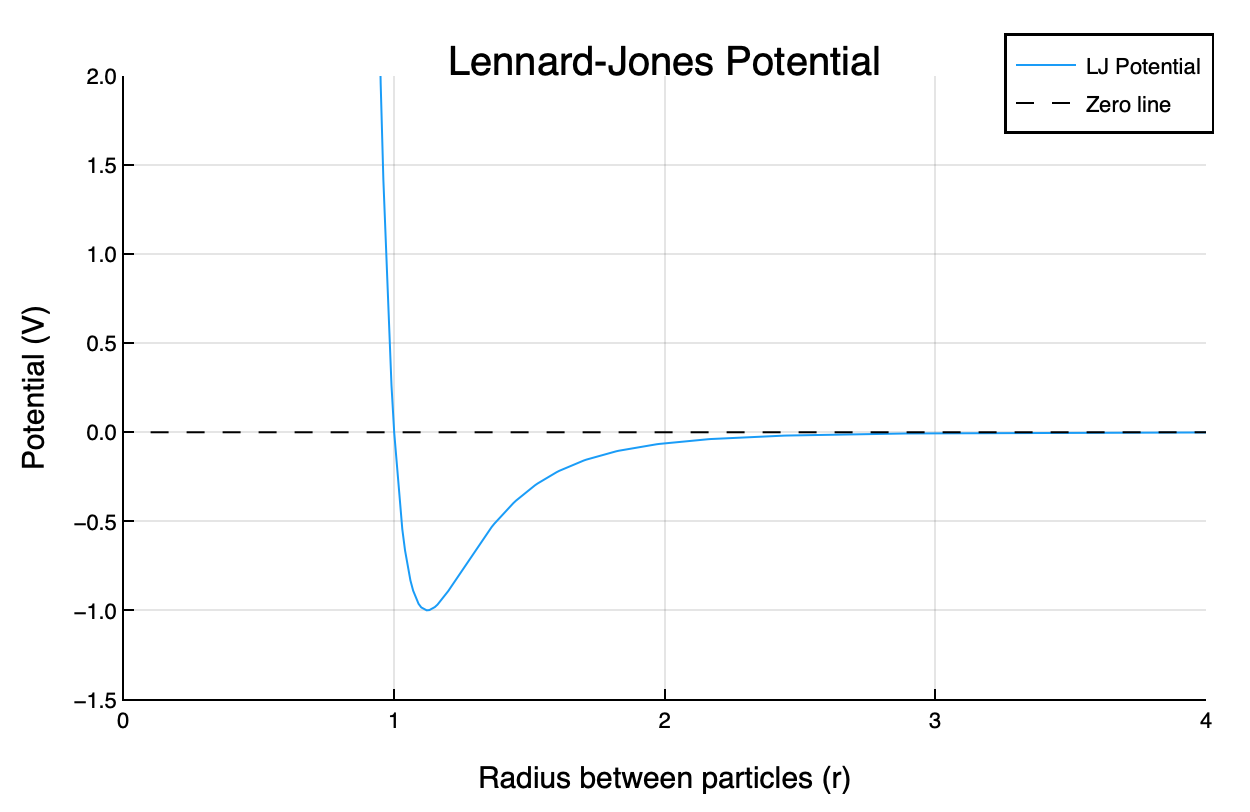
\includegraphics[scale = 0.5]{Figures/LJPotential}
\caption{The Lennard-Jones potential. A simple yet realistic model of intramolecular forces.
\label{fig:LJ}} 
\end{figure}

\par It can be recalled that the force from a potential is given by

\begin{equation} \label{eq:forceEq}
F = -\nabla U,
\end{equation}
and thus the force between two particles is zero at the bottom of the potential well. With that location as a reference, distances any greater will produce a force that is attractive and at any lesser distance the force is intensely repulsive.
\par Calculating the potential between two particles is not difficult; but finding the total potential energy of a system of several particles becomes increasingly computationaly expensive. Because of the simplicity of the Lennard-Jones potential, the computational power required to solve for the system's energy is still relatively small. In preparation for using real, quantum-mechanical data, each system's energy will be treated as expensive to compute. 



\section{Constructing a Model}\label{Sect:LJModels}
\par Ensuring a sufficient number and breadth of samples as well as reasonable basis functions becomes difficult as the number of dimensions goes beyond 2 or 3. Ways to determine quality of samples will be discussed later and from studying a variety of potential basis functions, Bessel functions of the second kind, $Y_\alpha(x)$, have the potential to be useful.
\par Rewriting eq. \ref{eq:Aby} in component form yields
\begin{equation}
\begin{bmatrix}
A_{11} & A_{12} & \ldots & A_{1m} \\
A_{21} \\
\vdots & & & \vdots\\
A_{n1} & \ldots & & A_{nm}
\end{bmatrix}
\begin{bmatrix}
b_0 \\
b_1 \\
b_2 \\
\vdots \\
b_m 
\end{bmatrix}
=
\begin{bmatrix}
V_1 \\
V_2 \\
V_3 \\ 
\vdots \\
V_n
\end{bmatrix}.
\label{eq:AMatrix}
\end{equation}
\par Recognizing each row of $\mathbf{A}$ as a unique configuration, eq. \ref{eq:AMatrix} can be written as a system of linear equations as follows
\begin{align}
A_{11}b_1 + A_{12}b_2 + A_{13}b_3 + ... + A_{1m}b_m &= V_1 \nonumber \\
A_{21}b_1 + A_{22}b_2 + A_{23}b_3 + ... + A_{2m}b_m &= V_2 \nonumber \\
A_{n1}b_1 + A_{n2}b_2 + A_{n3}b_3 + ... + A_{nm}b_m &= V_n.
\end{align}
where $V_n$ is the total potential energy of configuration $n$. Each element of matrix $\mathbf{A}$ will be populated as follows
\begin{align}
A_{11} &= Y_0(\alpha_{01} r_{12}) + Y_0(\alpha_{01} r_{13}) + Y_0(\alpha_{01} r_{23}) + \ldots \nonumber \\
A_{12} &= Y_0(\alpha_{02} r_{12}) + Y_0(\alpha_{02} r_{13}) + Y_0(\alpha_{02} r_{23}) + \ldots \nonumber \\
A_{1m} &= Y_0(\alpha_{0m} r_{12}) + Y_0(\alpha_{0m} r_{13}) + Y_0(\alpha_{0m} r_{23}) + \ldots \label{eq:fillBessel}
\end{align}
where $\alpha_{0m}$ is the $m$-th zero of $Y_0$, the zeroth Bessel function of the first kind. Each $r_{xy}$ represents the separation vector norm ($\ell^2$ norm) for a single particle, $x$, and its pair, $y$, in the configuration. Because this model only accepts the $\ell^2$ norm of each separation vector, it is only a simple distance-dependent model using pair-interactions rather than a more complicated model using three body interactions (see Section \ref{Sect:futureWork}).

\par An example of a random assortment of particles in a box can be seen in fig. \ref{fig:tenParticles}. If two particles are generated too close together, it will cause a large spike in the system's potential. Thus a minimum separation distance must be enforced for each configuration generated. This minimum separation distance will ensure some degree of uniformity in the configurations and their total potential, effectively reducing the range of possible energies and requiring fewer training systems. 

\begin{figure}%[h]
\centering
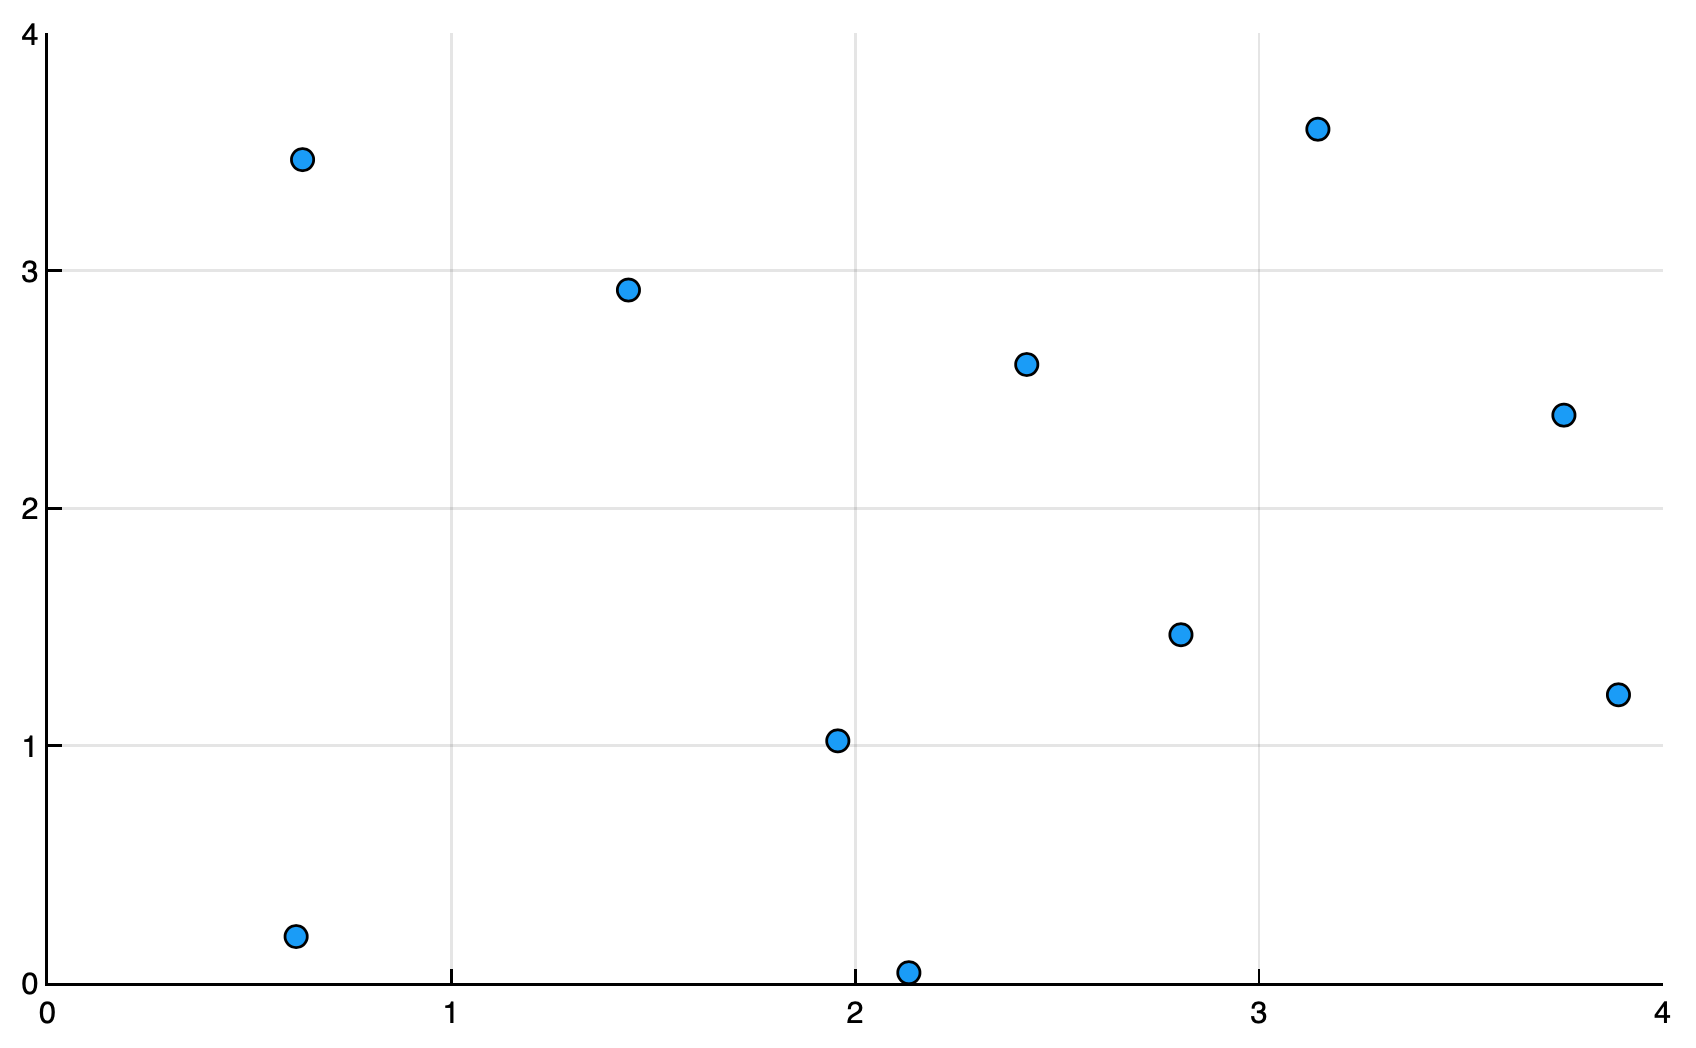
\includegraphics[scale = 0.4]{Figures/tenParticles}
\caption{A random assortment of 10 particles in a 4x4 square. No two particles are allowed to be within a pre-specified distance of each other. 
\label{fig:tenParticles}} 
\end{figure}

\par Through experimentation, the detailed relationship between size of the training set, number of basis functions, and the minimum separation distance can be outlined. In general, the accuracy of the model increases as the number of training sets and basis functions increases. The accuracy also increases when the minimum separation distance does not correspond to a particularly large potential energy. In the case of the Lennard-Jones potential in fig. \ref{fig:LJ}, the minimum separation distance has a preferred minimum of 0.8 or 0.9 to avoid large errors in the constructed model.



\section{Multi-Type Particle Systems}\label{Sect:diatomic}
\par Now that a simple monotomic model has been constructed, it can be adjusted to handle two different types of particles. The different particles can be labeled type-$A$ and type-$B$. This diatomic system will now require \textit{three} different potential equations, one describing each type of interaction. The three unique interactions are type-$A$ interacting with another type-$A$, a type-$A$ interacting with a type-$B$, and a type-$B$ with another type-$B$. Because these are arbitrary interactions (due to unspecified atomic structure), they can be defined by choosing reasonable values of $\varepsilon$ and $\sigma$ from eq. \ref{eq:LJ}. These constants will be chosen as follows
\begin{align}
V_{AB}(r) &= 4 \bigg[\Big(\frac{1}{r}\Big)^{12} - \Big(\frac{1}{r}\Big)^6\bigg] \label{LJ} \\
V_{AA}(r) &= 4 (0.7) \bigg[\Big(\frac{0.8}{r}\Big)^{12} - \Big(\frac{0.8}{r}\Big)^6\bigg] \label{LJ} \\
V_{BB}(r) &= 4 (0.4) \bigg[\Big(\frac{1.1}{r}\Big)^{12} - \Big(\frac{1.1}{r}\Big)^6\bigg] \label{LJ}.
\end{align}
The graph of each potential can be seen in fig. \ref{fig:3LJ}. Each of the equilibrium positions and energies is slightly different, but all in the same neighborhood.

\begin{figure}%[h]
\centering
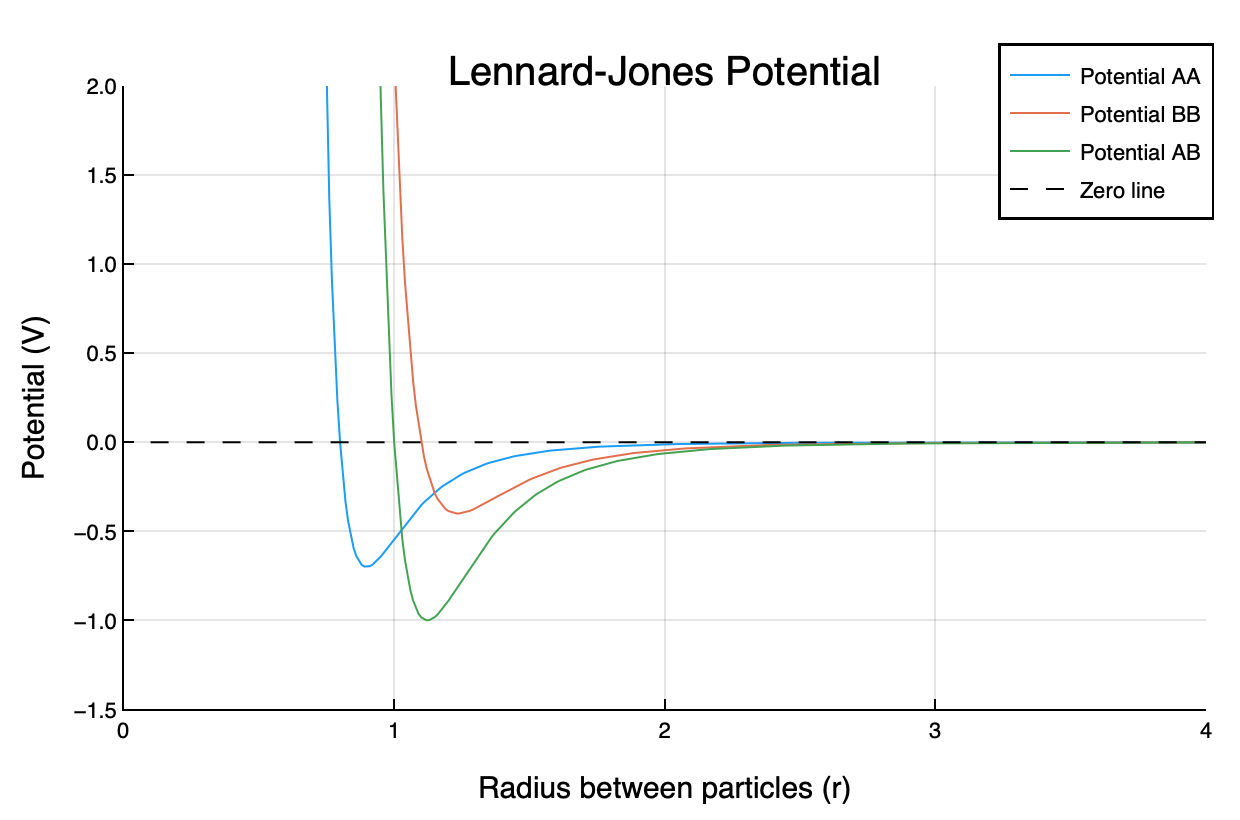
\includegraphics[scale = 0.5]{Figures/newLJPotential}
\caption{A Lennard-Jones potential for each particle interaction type (AA, AB, and BB). Each interaction potential has a slightly different equilibrium position and energy. 
\label{fig:3LJ}} 
\end{figure}

\par Due to this increase in complexity, matrix $\mathbf{A}$ will need to contain \textit{three} columns where the previous model had only one. Each column will represent one of the three interaction types. The problem of determining the particle type ratio must also be addressed. If the particle number (10) and box size ($4\times4$) remain constant, how many type-$A$ versus type-$B$ particles should there be to help train an effective model?
\par This question can be generalized to ask: what is a sufficient breadth of samples for this model? The answer depends greatly upon the desired range of predictions. As will be seen in Section \ref{Sect:procedureData}, the actual configurations vary in particle number and particle type ratio. Therefore, the model constructed here should be trained and tested using a spread of values for those two variables. Each training and testing set will thus be populated by a random number and ratio of particles. 
\par Once a model has been properly constructed and trained, its accuracy can be visually determined by plotting each system's predicted energy versus its actual energy. An example of this type of plot can be seen in fig. \ref{fig:diatomicAccuracy} and will be used again later on.

\begin{figure}%[h]
\centering
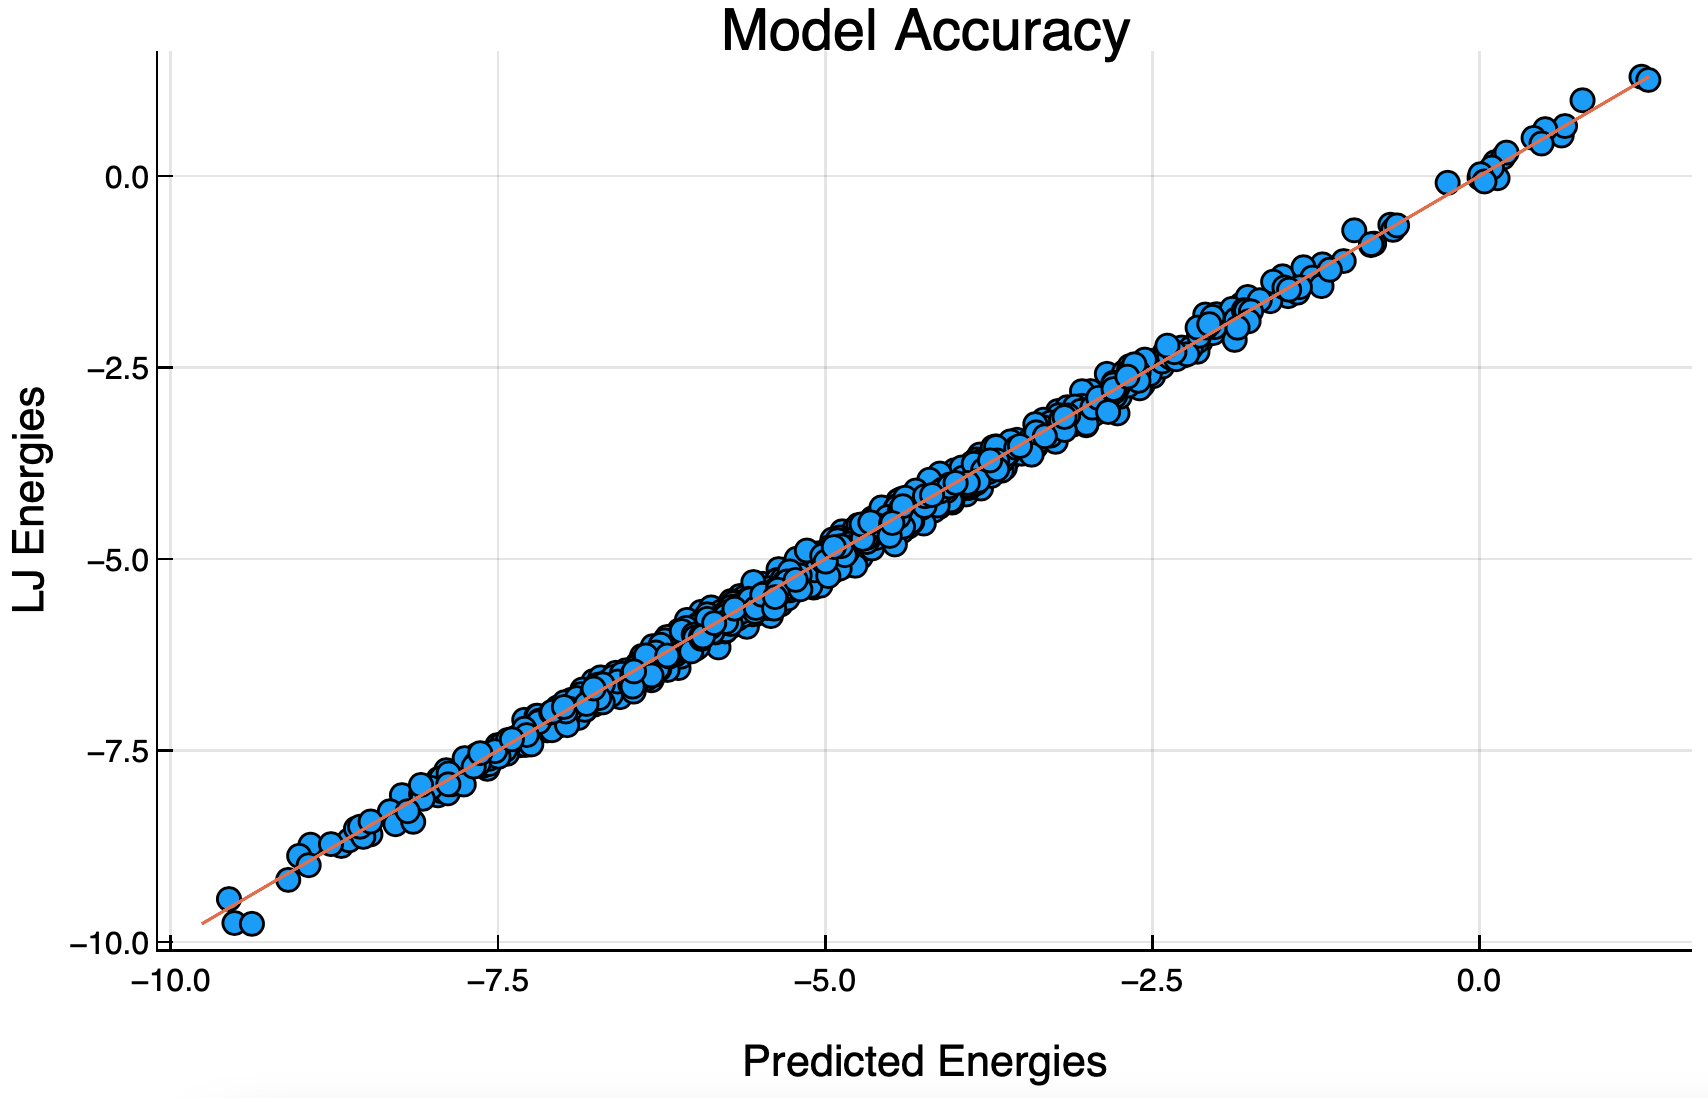
\includegraphics[scale = 0.4]{Figures/diatomicAccuracy}
\caption{1000 tests of a model with a training size of 300 systems, 900 total basis functions, and a spread of particle type ratios each for a 10 particle system. The fit is very good, denoting a highly accurate model.
\label{fig:diatomicAccuracy}}
\end{figure}

\par Now that a successful model has been created for a simplified potential, it can be adapted to fit real data in the hopes of producing useful data faster than current models.